\begin{enumerate}[label=\thechapter.\arabic*,ref=\thechapter.\theenumi]
\item Let a frequency modulated (FM) signal : $ x(t) = A \cos(\omega_c t + k_f \int_{-\infty}^{t} m(\lambda) d\lambda)$ , where $ m(t) $is a message signal of bandwidth $ W $. It is passed through a non-linear system with output $y(t) = 2x(t) + 5(x(t))^2 $.
Let $B_T $denote the FM bandwidth. The minimum value of $ \omega_c $ required to recover $ x(t) $ from $ y(t) $ is:\\
\begin{enumerate}[label = (\Alph*)]
\item $B_T + W$ \\
\item $\dfrac{3}{2} B_T$ \\
\item $2B_T + W$ \\
\item $\dfrac{5}{2} B_T$ \\
\end{enumerate}

\solution
\newpage

\item Let an input $x[n]$ having discrete-time Fourier transform
$X(e^{j\Omega}) = 1 - e^{-j\Omega} + 2e^{-3j\Omega}$
be passed through an LTI system. The frequency response of the LTI system is 
$H(e^{j\Omega}) = 1 - \frac{1}{2} e^{-2j\Omega}$
The output $y[n]$ of the system is \\ \hfill(GATE EC 2023)
\solution 
\input{2023/EC/48/ec48.tex}
\newpage
\item The Fourier transform $X(\omega)$ of $x(t) = e^{-t^2}$ is\\
Note:$\int_{-\infty}^{\infty} e^{-y^2} \,dy = \sqrt{\pi}$ \\  
A) $\sqrt{\pi} e^{\frac{\omega^2}{2}}$ \\
B) $\frac{e^{\frac{-\omega^2}{4}}}{2\sqrt{\pi}}$ \\
C) $\sqrt{\pi} e^{\frac{-\omega^2}{4}}$ \\
D) $\sqrt{\pi} e^{\frac{-\omega^2}{2}}$\\
\hfill Gate 2023 EC Question 28
\solution
\iffalse
\let\negmedspace\undefined
\let\negthickspace\undefined
\documentclass[a4,12pt,twocolumn]{IEEEtran}
%\documentclass[conference]{IEEEtran}
%\IEEEoverridecommandlockouts
% The preceding line is only needed to identify funding in the first footnote. If that is unneeded, please comment it out.
\usepackage{cite}
\usepackage{amsmath,amssymb,amsfonts,amsthm}
\usepackage{algorithmic}
\usepackage{graphicx}
\usepackage{textcomp}
\usepackage{xcolor}
\usepackage{txfonts}
\usepackage{listings}
\usepackage{enumitem}
\usepackage{mathtools}
\usepackage{gensymb}
\usepackage[breaklinks=true]{hyperref}
\usepackage{tkz-euclide} % loads  TikZ and tkz-base
\usepackage{listings}
\usepackage{empheq}
\usepackage[utf8]{inputenc}
\usepackage{pgfplots}
\usepackage{mathrsfs}
\usepackage{multicol}
\usepackage{array}
%\usepackage{setspace}
%\usepackage{gensymb}
%\doublespacing
%\singlespacing

%\usepackage{graphicx}

\DeclareMathOperator*{\Res}{Res}
%\renewcommand{\baselinestretch}{2}
\renewcommand\thesection{\arabic{section}}
\renewcommand\thesubsection{\thesection.\arabic{subsection}}
\renewcommand\thesubsubsection{\thesubsection.\arabic{subsubsection}}

\renewcommand\thesectiondis{\arabic{section}}
\renewcommand\thesubsectiondis{\thesectiondis.\arabic{subsection}}
\renewcommand\thesubsubsectiondis{\thesubsectiondis.\arabic{subsubsection}}

% correct bad hyphenation here
\hyphenation{op-tical net-works semi-conduc-tor}
\def\inputGnumericTable{}                                 %%

\lstset{
%language=C,
frame=single, 
breaklines=true,
columns=fullflexible
}
%\lstset{
%language=tex,
%frame=single, 
%breaklines=true
%}

\begin{document}
%


\newtheorem{theorem}{Theorem}[section]
\newtheorem{problem}{Problem}
\newtheorem{proposition}{Proposition}[section]
\newtheorem{lemma}{Lemma}[section]
\newtheorem{corollary}[theorem]{Corollary}
\newtheorem{example}{Example}[section]
\newtheorem{definition}[problem]{Definition}
%\newtheorem{thm}{Theorem}[section] 
%\newtheorem{defn}[thm]{Definition}
%\newtheorem{algorithm}{Algorithm}[section]
%\newtheorem{cor}{Corollary}
\newcommand{\BEQA}{\begin{eqnarray}}
\newcommand{\EEQA}{\end{eqnarray}}
\newcommand{\define}{\stackrel{\triangle}{=}}

\bibliographystyle{IEEEtran}
%\bibliographystyle{ieeetr}


\providecommand{\mbf}{\mathbf}
\providecommand{\pr}[1]{\ensuremath{\Pr\left(#1\right)}}
\providecommand{\qfunc}[1]{\ensuremath{Q\left(#1\right)}}
\providecommand{\sbrak}[1]{\ensuremath{{}\left[#1\right]}}
\providecommand{\lsbrak}[1]{\ensuremath{{}\left[#1\right.}}
\providecommand{\rsbrak}[1]{\ensuremath{{}\left.#1\right]}}
\providecommand{\brak}[1]{\ensuremath{\left(#1\right)}}
\providecommand{\lbrak}[1]{\ensuremath{\left(#1\right.}}
\providecommand{\rbrak}[1]{\ensuremath{\left.#1\right)}}
\providecommand{\cbrak}[1]{\ensuremath{\left\{#1\right\}}}
\providecommand{\lcbrak}[1]{\ensuremath{\left\{#1\right.}}
\providecommand{\rcbrak}[1]{\ensuremath{\left.#1\right\}}}
\theoremstyle{remark}
\newtheorem{rem}{Remark}
\newcommand{\sgn}{\mathop{\mathrm{sgn}}}
%\providecommand{\abs}[1]{\left\vert#1\right\vert}
\providecommand{\res}[1]{\Res\displaylimits_{#1}} 
%\providecommand{\norm}[1]{\left\lVert#1\right\rVert}
%\providecommand{\norm}[1]{\lVert#1\rVert}
\providecommand{\mtx}[1]{\mathbf{#1}}
%\providecommand{\mean}[1]{E\left[ #1 \right]}
\providecommand{\fourier}{\overset{\mathcal{F}}{ \rightleftharpoons}}
%\providecommand{\hilbert}{\overset{\mathcal{H}}{ \rightleftharpoons}}
\providecommand{\system}{\overset{\mathcal{H}}{ \longleftrightarrow}}
	%\newcommand{\solution}[2]{\textbf{Solution:}{#1}}
\newcommand{\solution}{\noindent \textbf{Solution: }}
\newcommand{\cosec}{\,\text{cosec}\,}
\providecommand{\dec}[2]{\ensuremath{\overset{#1}{\underset{#2}{\gtrless}}}}
\newcommand{\myvec}[1]{\ensuremath{\begin{pmatrix}#1\end{pmatrix}}}
\newcommand{\mydet}[1]{\ensuremath{\begin{vmatrix}#1\end{vmatrix}}}
%\numberwithin{equation}{section}
%\numberwithin{equation}{subsection}
%\numberwithin{problem}{section}
%\numberwithin{definition}{section}
%\makeatletter
%\@addtoreset{figure}{problem}
%\makeatother

%\let\StandardTheFigure\thefigure
\let\vec\mathbf

\title{
\Huge\textbf{Gate EE 2023}\\
\Huge\textbf{EE1205} Signals and Systems\\
}
\large\author{Nimal Sreekumar\\EE23BTECH11044}

% make the title area
\maketitle


%\tableofcontents

\bigskip

\renewcommand{\thefigure}{\arabic{figure}}
\renewcommand{\thetable}{\theenumi}
%\renewcommand{\theequation}{\theenumi}


\textbf{Question Gate 2023 EE:}
For the signals x\brak{t} and y\brak{t} shown in the figure, $z\brak{t}=x\brak{t}*y\brak{t}$ is maximum at $t=T_1$. Then $T_1$ in seconds is .......... \brak{\text{Round off to the nearest integer}}\\

\begin{tikzpicture}
\begin{axis}[xmin=-3, xmax=7, ymin=-3, ymax=3, axis lines=middle, xlabel={$t$}, title={$y\brak{t}$}]
 \addplot[blue] coordinates {(-3,0) (1,0)};
  \addplot[blue] coordinates {(1,0) (1,-2)};
   \addplot[dashed] coordinates {(0,-2) (1,-2)};
  \addplot[blue, domain=1:5] {x - 3};
  \addplot[blue] coordinates {(5,2) (5,0)};
  \addplot[blue] coordinates {(5,0) (7,0)};
  \addplot[dashed] coordinates {(0,2) (5,2)};
    \end{axis}
\end{tikzpicture}

\begin{tikzpicture}
    \begin{axis}[xmin=-3, xmax=3, ymin=-3, ymax=3, axis lines=middle, xlabel={$t$} ,title={$x\brak{t}$}]
        \addplot[blue] coordinates {(-3,0) (-1,0)};
        \addplot[blue] coordinates {(-1,0) (-1,1)};
        \addplot[blue] coordinates {(-1,1) (1,1)};
        \addplot[blue] coordinates {(1,1) (1,0)};
        \addplot[blue] coordinates {(1,0) (3,0)};
    \end{axis}
\end{tikzpicture}

\hfill (GATE EE 2023)
\solution
\fi

\begin{table}[htbp]
\centering
\renewcommand\thetable{1}
\begin{tabular}{|c|m{3.5cm}|m{3cm}|}
    \hline
    \textbf{Variable} & \textbf{values} & \textbf{Description} \\
    \hline
    $x\brak{t}$ & $u\brak{t+1}-u\brak{t-1}$ & signal 1\\
    \hline
    $ y\brak{t} $ & $y\brak{t} = 
    \begin{cases}
        t-3 & ; 1\leq n \leq 5 \\
        0 & ; otherwise \\
    \end{cases}$ & signal 2\\
    \hline
    $X\brak{s}$ & $\int_{0}^{\infty}x\brak{t}e^{-st}dt$ & Laplace transform of $x\brak{t}$\\
    \hline
   $Y\brak{s}$ & $\int_{0}^{\infty}y\brak{t}e^{-st}dt$ & Laplace transform of $y\brak{t}$ \\
    \hline
    $\mathscr{L^{-1}} \{Z(s)\}$ &$f\brak{t-c}u\brak{t-c}=\mathscr{L^{-1}}\brak{e^{-cs}F\brak{s}} $& Inverse Laplace transform \\
    \hline
\end{tabular}
\caption{Input Parameters}
\label{tab:11.9.5.32}
\end{table}

Using laplace transform,
\begin{align}
z\brak{t} &=x\brak{t}*y\brak{t}\label{eq:gate_ee_Q31.1} \\
Z\brak{s} &=X\brak{s}Y\brak{s}\label{eq:gate_ee_Q31.2} \\
X\brak{s} &= \frac{1}{s} \brak{e^{s}-e^{-s}} \label{eq:gate_ee_Q31.3}\\
Y\brak{s} &= \frac{2s+1}{s^2} \brak{e^{-s}-e^{-5s}}\label{eq:gate_ee_Q31.4}\\
Z\brak{s} &= \frac{2s+1}{s^3} \brak{1-e^{-4s}-e^{-2s}+e^{-6s}}\label{eq:gate_ee_Q31.5}
\end{align}
Now taking inverse laplace transform for each terms, $\mathscr{L^{-1}} \{Z(s)\}$
\begin{align}
&= \left( 2t + \frac{t^2}{2} \right) u(t) \nonumber \\
&\quad - \left( 2(t-4) + \frac{(t-4)^2}{2} \right)u(t-4) \nonumber \\
&\quad - \left( 2(t-2) + \frac{(t-2)^2}{2} \right)u(t-2) \nonumber \\
&\quad + \left( 2(t-6) + \frac{(t-6)^2}{2} \right)u(t-6) \nonumber
\end{align}\label{eq:gate_ee_Q31.6}
From the plot it is clear that $T_1=4$.\\
\begin{figure}[h]
\centering
   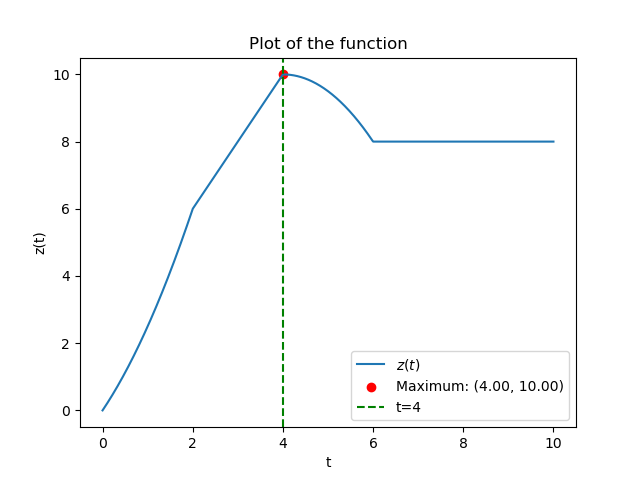
\includegraphics[width=1\linewidth]{2023/EE/31/figs/figs/gate2023EE.png}
   \caption{z\brak{t} vs. t}
   \label{fig:gate2023EE1}
 \end{figure}\\
Now in time domain,
 \begin{align}
z\brak{t} &=x\brak{t}*y\brak{t} = y\brak{t}*x\brak{t}\label{eq:gate_ee_Q31.7}\\
z\brak{t} &=\int_{-\infty}^{\infty} y\brak{\tau}x\brak{t-\tau}d\tau\label{eq:gate_ee_Q31.8}
\end{align}
$x\brak{\tau}$ is an even signal,
\begin{align}
x\brak{\tau}= x\brak{-\tau}\label{eq:gate_ee_Q31.9}\\
 x\brak{-\tau}= 
    \begin{cases}
        1 & ; -1\leq -\tau \leq 1 \\
        0 & ; \text{otherwise} \\
    \end{cases}\label{eq:gate_ee_Q31.10}
    \end{align}
    
    \begin{align}
    x\brak{-\tau} \xleftrightarrow{\text{Time shifting}} x\brak{t-\tau}\label{eq:gate_ee_Q31.11} \\
    x\brak{t-\tau}= 
    \begin{cases}
        1 & ; t-1\leq t-\tau \leq t+1 \\
        0 & ; \text{otherwise} \\
    \end{cases}\label{eq:gate_ee_Q31.12}
\end{align}\\
For $z\brak{t}$ to be maximum both $y\brak{\tau}$ and $x\brak{t-\tau}$ must be maximum,
\begin{align}
\implies t-1 &= 3 \quad \text{or} \quad t+1 = 5 \nonumber \\
t &= T_1 = 4 \nonumber
\end{align}

\newpage

 \item Let $x(t) = 10 \cos(10.5 \omega t)$ be passed through an LTI system with impulse response $h(t) = \pi\left(\frac{\sin(\omega t)}{\pi t}\right)^2 \cos(10 \omega t)$ . The output of the system is:\\ \hfill(GATE EC 2023)\\
A) $\frac{15}{4}\omega \cos(10.5 \omega t)$ \\
B) $\frac{15}{2}\omega \cos(10.5 \omega t)$ \\
C) $\frac{15}{8}\omega \cos(10.5 \omega t)$ \\
D) $15\omega \cos(10.5 \omega t)$ \\
 \solution
\documentclass[journal,12pt,twocolumn]{IEEEtran}

% Packages
\usepackage{cite}
\usepackage{amsmath,amssymb,amsfonts,amsthm}
\usepackage{graphicx}
\usepackage{textcomp}
\usepackage{xcolor}
\usepackage{txfonts}
\usepackage{listings}
\usepackage{enumitem}
\usepackage{mathtools}
\usepackage{float}
\usepackage{gensymb}
\usepackage{comment}
\usepackage{hyperref}
\usepackage{tkz-euclide}
\usepackage{gvv}
\usepackage[latin1]{inputenc}
\usepackage{color}
\usepackage{array}
\usepackage{longtable}
\usepackage{calc}
\usepackage{multirow}
\usepackage{hhline}
\usepackage{ifthen}
\usepackage{lscape}
\usepackage{subcaption}
\usepackage{tikz}
\usepackage{circuitikz}
\usepackage{wrapfig}
\usepackage{lipsum}
\usepackage[export]{adjustbox}
\usepackage{inputenc}

% Custom commands and macros
\newtheorem{theorem}{Theorem}[section]
\newtheorem{problem}{Problem}
\newtheorem{proposition}{Proposition}[section]
\newtheorem{lemma}{Lemma}[section]
\newtheorem{corollary}[theorem]{Corollary}
\newtheorem{example}{Example}[section]
\newtheorem{definition}[problem]{Definition}
\newtheorem{rem}{Remark}
\newcommand{\BEQA}{\begin{eqnarray}}
\newcommand{\EEQA}{\end{eqnarray}}
\newcommand{\define}{\stackrel{\triangle}{=}}
\renewcommand{\thefigure}{\theenumi}
\renewcommand{\thetable}{\theenumi}



\begin{document}

\title{GATE 2023 EC 49}
\author{EE23BTECH11045 - Palavelli Srija$^{*}$}
\maketitle

\bigskip

\textbf{Question 12.7.7:} 
Let $x(t) = 10 \cos(10.5 \omega t)$ be passed through an LTI system with impulse response $h(t) = \pi\left(\frac{\sin(\omega t)}{\pi t}\right)^2 \cos(10 \omega t)$ . The output of the system is: \\

\textbf{Solution:}
\begin{table}[h!]
    \centering
    \begin{table}[htbp]
	\centering
	\noindent
	\fontsize{10}{15}\selectfont {
		\resizebox{0.45\textwidth}{!}{%
			\begin{tabular}{|c|c|c|}
				\hline
				\textbf{Parameter} & \textbf{Value} & \textbf{Description} \\
				\hline
				$x\brak t$ & - & Input voltage \\
				\hline
				$y\brak t$ & - & Output voltage \\
				\hline
				$h\brak t$ & $\frac{y\brak t}{x\brak t}$ & Impulse response \\
				\hline
				$X\brak s$ & - & Input voltage in s-domain \\
				\hline
				$Y\brak s$ & - & Output voltage in s-domain \\
				\hline
				$H\brak s$ & $\frac{Y\brak s}{X\brak s}$ & Impulse response in s-domain \\
				\hline
			\end{tabular}
	} }
	\caption*{Input Table}
	
\end{table}
    \caption{Input Parameters}
    \label{tab:table_sr10}
\end{table}

Given \(h(t)\) is real and even. When a sinusoidal input is applied to an LTI system with an even impulse response, the output will also be sinusoidal. Hence, \(y(t) = A\cdot 10\cos(10.5 \omega t + \theta)\).

\[
x(t) \xrightarrow{\text{}} \boxed{\text{h(t)}} \xrightarrow{\text{}} y(t)
\]

\begin{align}
\text{Let } f(t) &= \pi\left(\frac{\sin(\omega t)}{\pi t}\right)^2 \\
h(t) &= f(t) \cos(10 \omega t)
\end{align}

Using 
\begin{align}
x_1(t) \cdot x_2(t) \xleftrightarrow{\mathcal{F}} X_1(\omega) * X_2(\omega)\\
\left(\frac{\sin(\omega t)}{\pi t}\right) \cdot \left(\frac{\sin(\omega t)}{\pi t}\right) \xleftrightarrow{\mathcal{F}} X_1(\omega) * X_2(\omega)
\end{align}
\begin{figure}[h!]
    \centering
    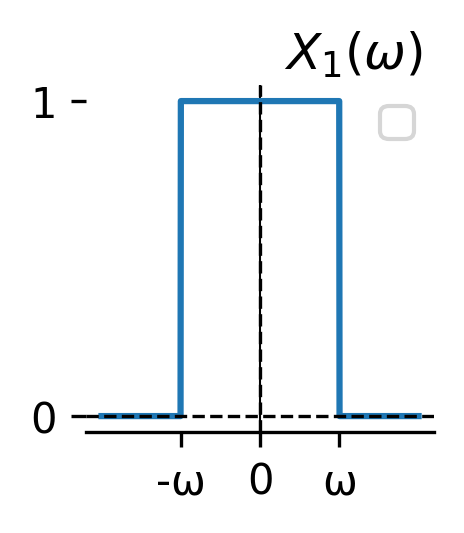
\includegraphics[width=0.4\columnwidth, height=2.5cm]{figs/plot.png}\hfill
    \begin{tabular}{c}
        {\sffamily\raisebox{1.75cm}{*}} 
    \end{tabular}\hfill
    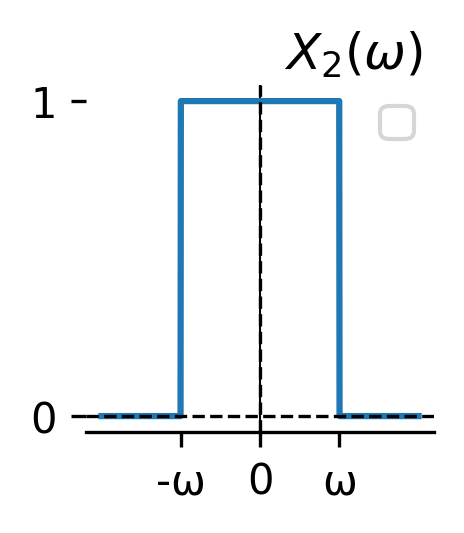
\includegraphics[width=0.4\columnwidth, height=2.5cm]{figs/plot4.png}
    
    \caption{}
    \label{fig:overall}
\end{figure}

\begin{align}
\left(\frac{\sin(\omega t)}{\pi t}\right)^2  \xleftrightarrow{\mathcal{F}} X_3(\omega) 
\end{align}
\begin{figure}[h!]
    \centering
    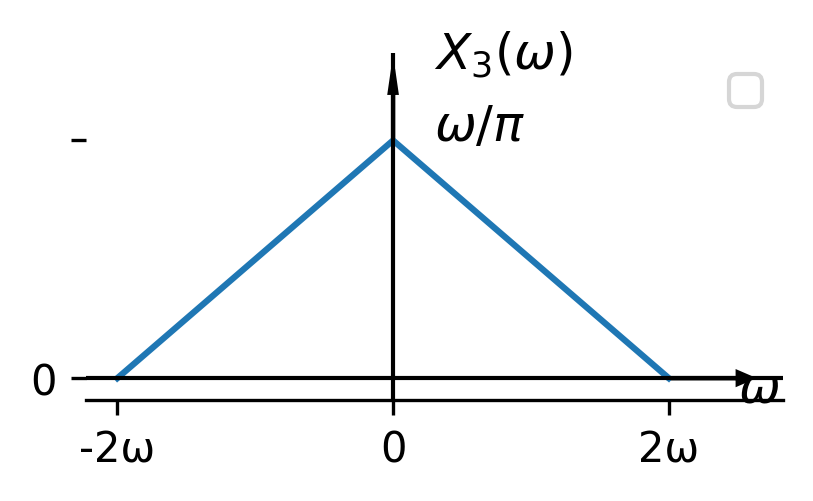
\includegraphics[width=0.5\columnwidth, height=3cm]{figs/plot1.png}
    \caption{}
    \label{fig:sr11}
\end{figure}
\begin{align}
\pi\left(\frac{\sin(\omega t)}{\pi t}\right)^2 \xleftrightarrow{\mathcal{F}} X_4(\omega)
\end{align}
\begin{figure}[h!]
    \centering
    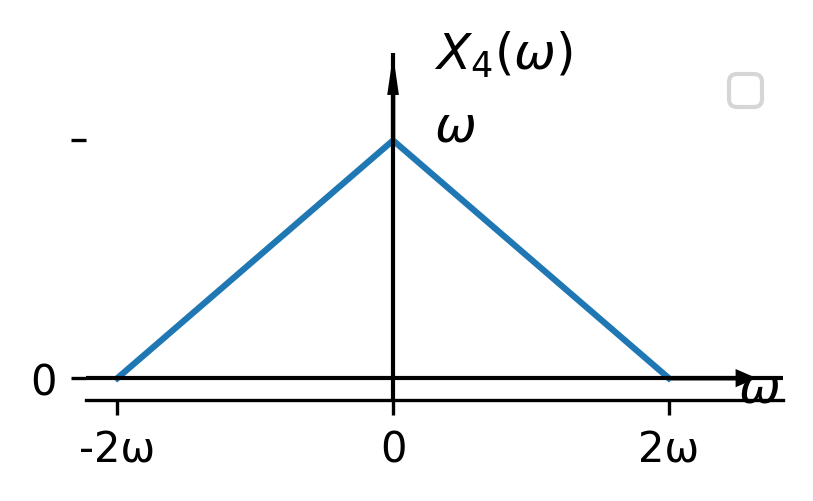
\includegraphics[width=0.5\columnwidth, height=3cm]{figs/plot2.png}
    \caption{}
    \label{fig:sr12}
\end{figure}
    \begin{align}
\text{From modulating property:} \nonumber \\
        f(t) \cos(\omega_0 t) \xleftrightarrow{\mathcal{F}} \frac{1}{2} \left[F(\omega + \omega_0) + F(\omega - \omega_0)\right]
    \end{align}

    \begin{align}
        H(\omega) &= \frac{1}{2} \left[F(\omega + 10\omega) + F(\omega - 10\omega)\right]
    \end{align}

\begin{figure}[h!]
    \centering
    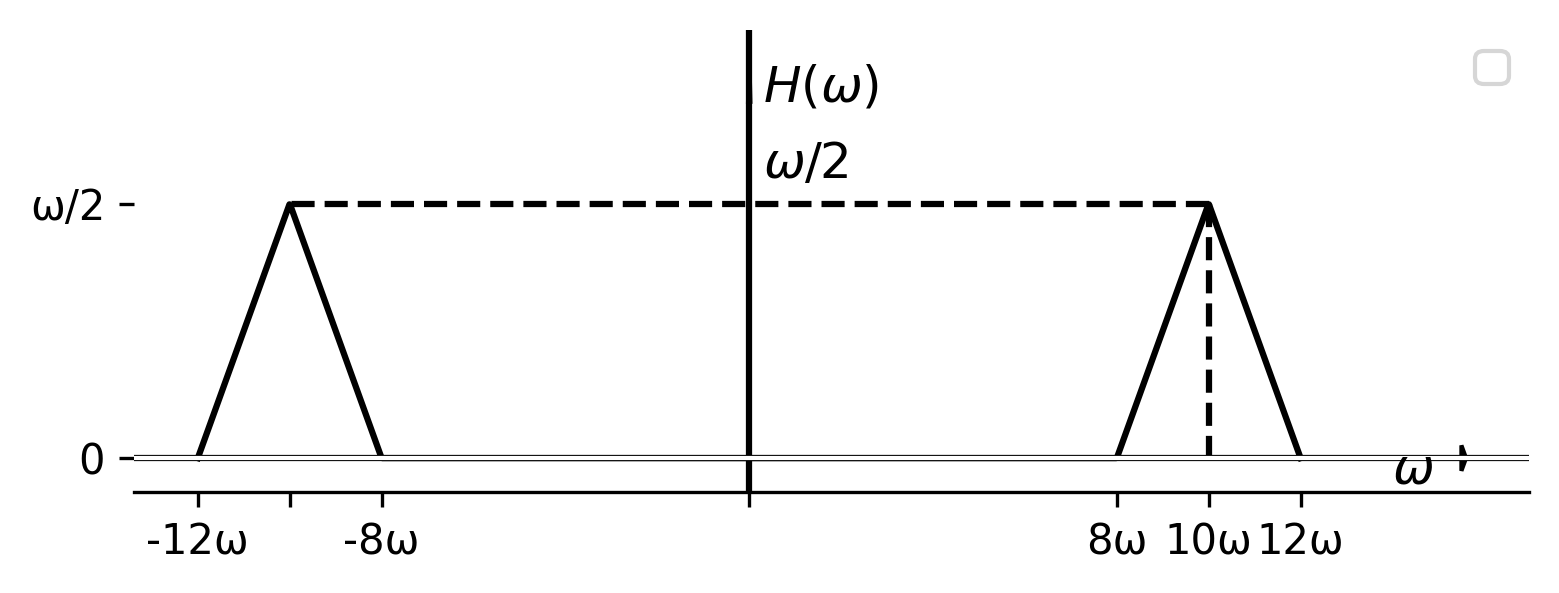
\includegraphics[width=0.7\columnwidth,height=2.5cm]{figs/plot3.png}
    \caption{}
    \label{fig:sr13}
\end{figure}
\begin{equation}
    \frac{\frac{\omega}{2} - 0}{10\omega - 12\omega} = \frac{|H(10.5\omega)| - 0}{10.5\omega - 12\omega}
\end{equation}

\begin{align}
A = |H(10.5\omega)| &= \frac{3}{8}\omega \quad \text{and} \quad  \theta= \angle H(10.5\omega) = 0^\circ
\end{align}

The output \(y(t)\):
\begin{align}
y(t) &= \frac{3}{8}\omega \cdot 10 \cos(10.5 \omega t) \\
&= \frac{15}{4}\omega \cos(10.5 \omega t)
\end{align}
\begin{figure}[h!]
    \centering
    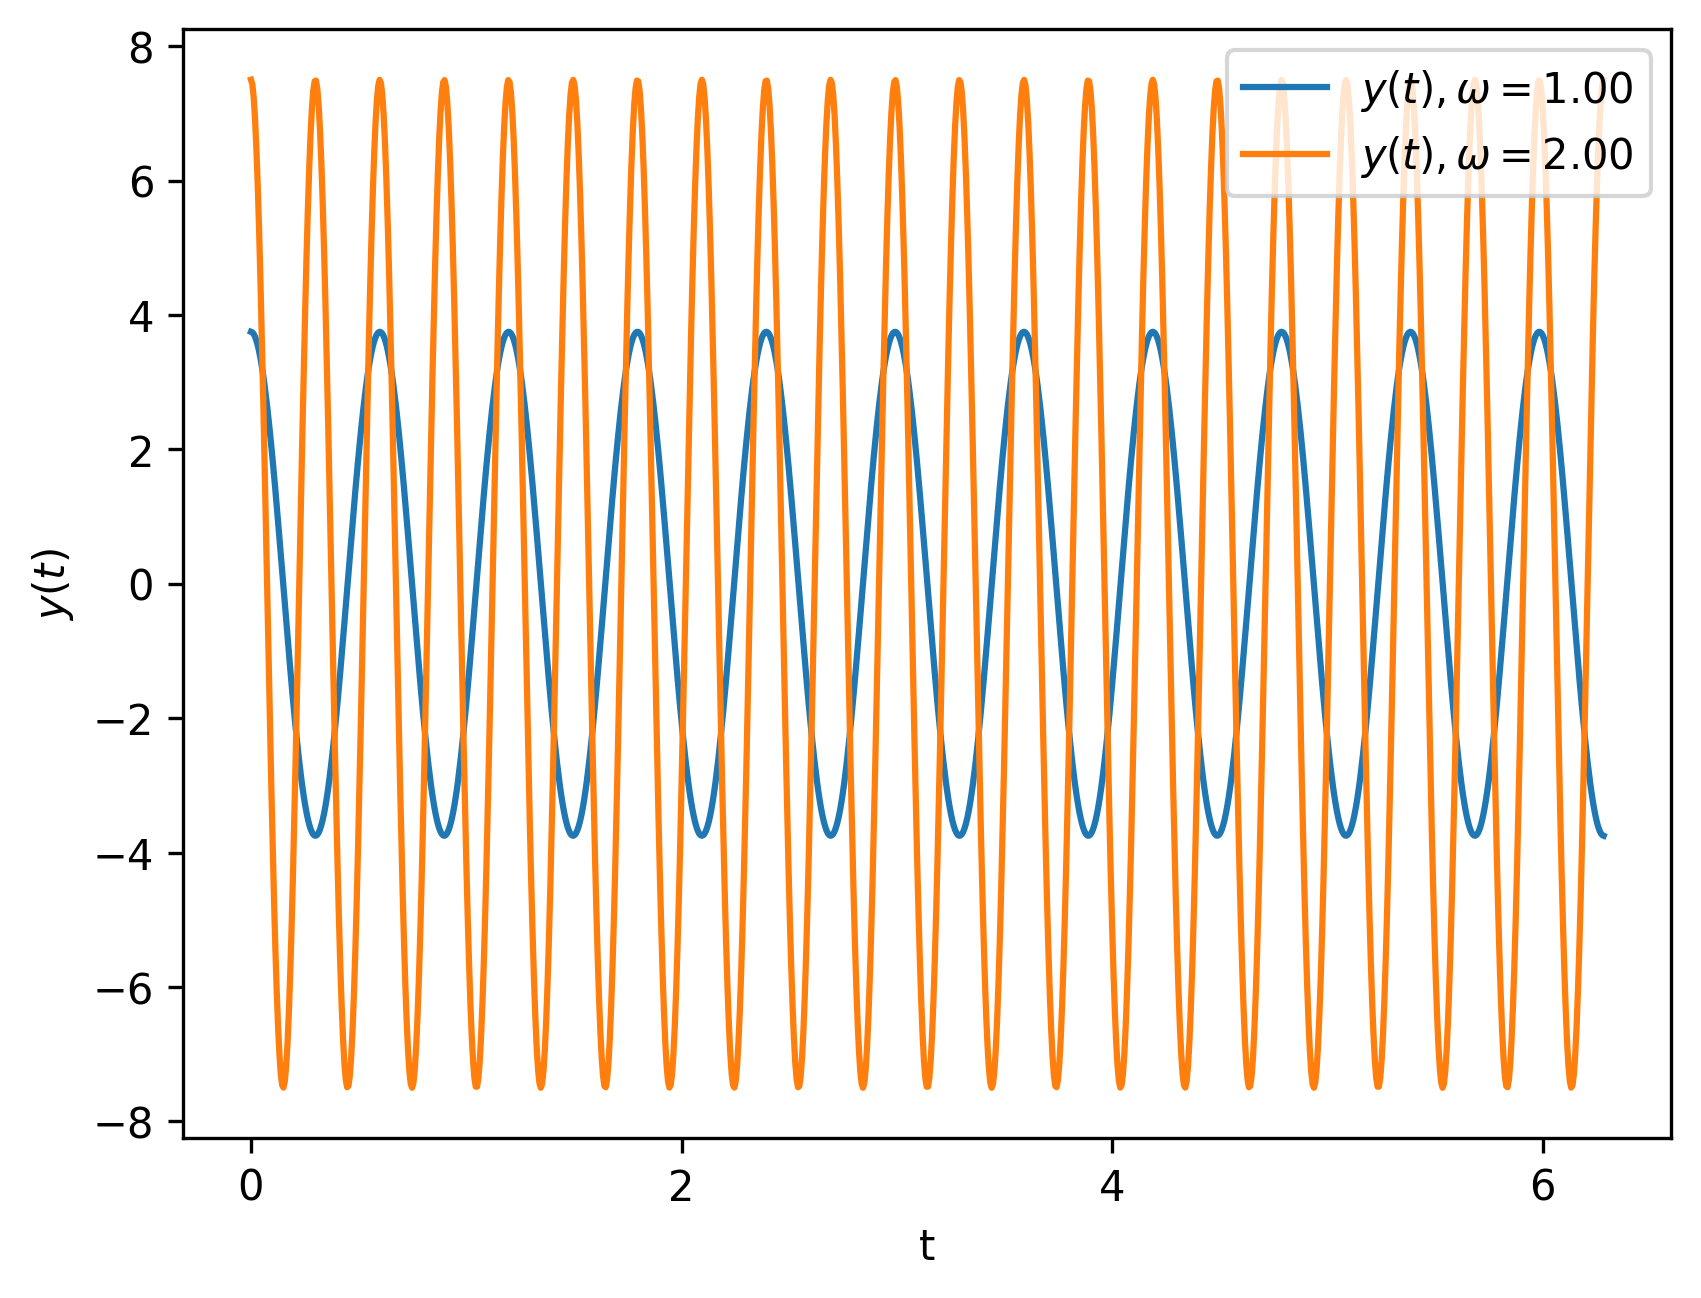
\includegraphics[width=\columnwidth]{figs/plot5.png}
    \caption{}
    \label{fig:sr14}
\end{figure}
\end{document}


\newpage
 
 \item Q27) Let m\brak{\text{t}} be a strictly band-limited signal with bandwidth B and energy E. Assuming $\omega_0$ = 10B, the energy in the signal $\text{m}\brak{\text{t}}\text{cos}\brak{\omega_0\text{t}}$\\[1ex]
\brak{\text{A}}\ $\frac{\text{E}}{4}$\\[1ex]
\brak{\text{B}}\ $\frac{\text{E}}{2}$\\[1ex]
\brak{\text{C}}\ \text{E}\\[1ex]
\brak{\text{D}}\ 2\text{E} \qquad\qquad\qquad\quad\qquad\qquad\qquad\qquad\brak{\text{GATE EC 2023}}

\solution
\iffalse
\let\negmedspace\undefined
\let\negthickspace\undefined
\documentclass[journal,12pt,twocolumn]{IEEEtran}
\usepackage{cite}
\usepackage{amsmath,amssymb,amsfonts,amsthm}
\usepackage{algorithmic}
\usepackage{graphicx}
\usepackage{textcomp}
\usepackage{xcolor}
\usepackage{txfonts}
\usepackage{listings}
\usepackage{enumitem}
\usepackage{mathtools}
\usepackage{gensymb}
\usepackage{comment}
\usepackage[breaklinks=true]{hyperref}
\usepackage{tkz-euclide} 
\usepackage{listings}
\usepackage{gvv}                                    
\usepackage{tikz}
\usepackage{pgfplots}
\def\inputGnumericTable{}                                 
\usepackage[latin1]{inputenc}                                
\usepackage{color}                                            
\usepackage{array}                                            
\usepackage{longtable}                                       
\usepackage{calc}                                             
\usepackage{multirow}                                         
\usepackage{hhline}                                           
\usepackage{ifthen}                                           
\usepackage{lscape}
\newtheorem{theorem}{Theorem}[section]
\newtheorem{problem}{Problem}
\newtheorem{proposition}{Proposition}[section]
\newtheorem{lemma}{Lemma}[section]
\newtheorem{corollary}[theorem]{Corollary}
\newtheorem{example}{Example}[section]
\newtheorem{definition}[problem]{Definition}
\newcommand{\BEQA}{\begin{eqnarray}}
\newcommand{\EEQA}{\end{eqnarray}}
\newcommand{\define}{\stackrel{\triangle}{=}}
\theoremstyle{remark}
\newtheorem{rem}{Remark}
\begin{document}
% Define custom function M(f)
\pgfmathdeclarefunction{Mf}{1}{%
  \pgfmathparse{sin(deg(#1))}%
}

\parindent 0px
\bibliographystyle{IEEEtran}

\title{GATE - EC 27}
\author{EE23BTECH11215 - Penmetsa Srikar Varma$^{}$% <-this % stops a space
}
\maketitle
\newpage
\bigskip

\renewcommand{\thefigure}{\theenumi}
\renewcommand{\thetable}{\theenumi}
\section*{Question}
Q27) Let m\brak{\text{t}} be a strictly band-limited signal with bandwidth B and energy E. Assuming $\omega_0$ = 10B, the energy in the signal $\text{m}\brak{\text{t}}\text{cos}\brak{\omega_0\text{t}}$\\[1ex]
\brak{\text{A}}\ $\frac{\text{E}}{4}$\\[1ex]
\brak{\text{B}}\ $\frac{\text{E}}{2}$\\[1ex]
\brak{\text{C}}\ \text{E}\\[1ex]
\brak{\text{D}}\ 2\text{E} \qquad\qquad\qquad\quad\qquad\qquad\qquad\qquad\brak{\text{GATE EC 2023}}
\section*{Solution}
\fi
\begin{table}[h]
    \centering
    \begin{tabular}{|c|c|c} 
    \hline
        Variables & Conditions \\
    \hline
        M\brak{\text{f}} & Fourier transform of m\brak{\text{t}}\\
    \hline
         \text{y}\brak{\text{t}} & \text{y}\brak{\text{t}}=$\text{m}\brak{\text{t}}\text{cos}\brak{2\pi\text{f}_0\text{t}}$\\
    \hline
        Y\brak{\text{f}} & Fourier transform of y\brak{\text{t}}\\
    \hline
    \end{tabular}

    \label{tab:my_label}
\end{table}
\begin{center}
    Table of Parameters\\
\end{center}
Let us assume for a case of M\brak{\text{f}},\\[1ex]
\begin{tikzpicture}
\begin{axis}[
    xlabel={f},
    ylabel={M\brak{\text{f}}},
    xmin=-1.5, xmax=1.5,
    ymin=0, ymax=1.2,
    axis lines=middle,
    minor tick num=1,
    width=10cm,
    height=6cm,
    xtick={-1,0,1},
    xticklabels={$-\text{B}$, 0, $\text{B}$},
    extra x ticks={-2,2},
    extra x tick labels={$-2B$, $2B$},
    extra x tick style={grid=none}
]
\addplot[blue, thick, domain=-1:1, samples=100] {1};
\draw[dotted] (axis cs:1,0) -- (axis cs:1,1);
\draw[dotted] (axis cs:-1,0) -- (axis cs:-1,1);
\end{axis}
\end{tikzpicture}\\[1ex]
Energy \brak{\text{E}} of the signal M\brak{\text{f}} is given by,
\begin{align}
\label{1}
    \text{E}&=\frac{1}{2\pi}\int_{-\text{B}}^{\text{B}}\abs{\text{M}\brak{\text{f}}}^2 \text{df}=\frac{\text{B}}{\pi}
\end{align}
Fourier transform of y\brak{\text{t}} is given by,
\begin{align}
    \text{Y}\brak{\text{f}}=\text{M}\brak{\text{f}}*\frac{1}{2}\brak{\delta\brak{\text{f}+\text{f}_0}+\delta\brak{\text{f}-\text{f}_0}}
\end{align}
\begin{align}
    \text{Y}\brak{\text{f}}=\frac{1}{2}\brak{\text{M}\brak{\text{f}+\text{f}_0}+\text{M}\brak{\text{f}-\text{f}_0}}
\end{align}
    
\begin{tikzpicture}[x=0.42cm, y=3cm] % Adjust the scale as needed
    % Axis
    \draw[->] (-12,0) -- (12,0) node[right] {f};
    \draw[->] (0,0) -- (0,1.5) node[above] {Y\brak{\text{f}}};
    
    % Horizontal lines
    \draw[line width=1.5pt] (-11,0.5) -- (-9,0.5);
    \draw[line width=1.5pt] (9,0.5) -- (11,0.5);
    
    % Labels
    \node[below] at (-11,0) {$-11\text{B}$};
    \node[below] at (-9,0) {$-9\text{B}$};
    \node[below] at (9,0) {$9\text{B}$};
    \node[below] at (11,0) {$11\text{B}$};
    
    % Set y-axis limits
    \draw[dashed] (-12,0.5) -- (12,0.5) node[right] {$\frac{1}{2}$};
    
    % Vertical dotted lines
    \draw[dotted] (-11,0) -- (-11,0.5);
    \draw[dotted] (-9,0) -- (-9,0.5);
    \draw[dotted] (9,0) -- (9,0.5);
    \draw[dotted] (11,0) -- (11,0.5);
\end{tikzpicture}\\[1ex]

Energy $\brak{\text{E}_1}$ of the signal Y\brak{\text{f}} is given by,
\begin{align}
\label{2}
    \text{E}_1&=\frac{1}{2\pi}\brak{\frac{2\text{B}}{4}+\frac{2\text{B}}{4}}=\frac{\text{B}}{2\pi}
\end{align}
So, from \brak{\ref{1}} and \brak{\ref{2}},
\begin{align}
    \text{E}_1&=\frac{\text{E}}{2}
\end{align}
Hence, option B is correct

\newpage

\item The following function is defined over the interval $[-L,L]:$
    $$f\brak{x}=px^4+qx^5$$
It is expressed as a Fourier series,
    $$f\brak{x}=a\brak{0}+\sum_{n=1}^{\infty}\cbrak{a\brak{n}\sin\brak{\frac{\pi x}{L}}+b\brak{n}\cos\brak{\frac{\pi x}{L}}}$$

which options amongst the following are true?
\begin{enumerate}[label=(\alph*)]
    \item $a\brak{n}$, $n=1,2,..,\infty$ depend on $p$
    \item $a\brak{n}$, $n=1,2,..,\infty$ depend on $q$
    \item $b\brak{n}$, $n=1,2,..,\infty$ depend on $p$
    \item $b\brak{n}$, $n=1,2,..,\infty$ depend on $q$
\end{enumerate}
\hfill(GATE 2023 CE Question 25)\\
\solution
\iffalse
\let\negmedspace\undefined
\let\negthickspace\undefined
\documentclass[journal,12pt,twocolumn]{IEEEtran}
\usepackage{cite}
\usepackage{amsmath,amssymb,amsfonts}
\usepackage{graphicx}
\usepackage{textcomp}
\usepackage{xcolor}
\usepackage{txfonts}
\usepackage{listings}
\usepackage{enumitem}
\usepackage{mathtools}
\usepackage{gensymb}
\usepackage{comment}
\usepackage[breaklinks=true]{hyperref}
\usepackage{tkz-euclide} 
\usepackage{listings}
\usepackage{gvv}                                        
\def\inputGnumericTable{}                                 
\usepackage[latin1]{inputenc}                                
\usepackage{color}                                            
\usepackage{array}                                            
\usepackage{longtable}                                       
\usepackage{calc}                                             
\usepackage{multirow}                                         
\usepackage{hhline}                                           
\usepackage{ifthen}                                           
\usepackage{lscape}
\usepackage[export]{adjustbox}

\newtheorem{theorem}{Theorem}[section]
\newtheorem{problem}{Problem}
\newtheorem{proposition}{Proposition}[section]
\newtheorem{lemma}{Lemma}[section]
\newtheorem{corollary}[theorem]{Corollary}
\newtheorem{example}{Example}[section]
\newtheorem{definition}[problem]{Definition}
\newcommand{\BEQA}{\begin{eqnarray}}
\newcommand{\EEQA}{\end{eqnarray}}
\newcommand{\define}{\stackrel{\triangle}{=}}
\newtheorem{rem}{Remark}

\begin{document}
\parindent 0px
\bibliographystyle{IEEEtran}

\vspace{3cm}

\title{}
\author{EE23BTECH11042 -  Khusinadha Naik$^{*}$
}
\maketitle
\newpage
\bigskip

% \renewcommand{\thefigure}{\theenumi}
% \renewcommand{\thetable}{\theenumi}


\noindent \textbf{26.} \hspace{2pt}A causal, discrete time system is described by the difference equation $y[n] = 0.5 y[n-1] + x[n]$, for all $n$, where $y[n]$ denotes the output sequence and $x[n]$ denotes the input sequence. Which of the following statements is/are TRUE?
\begin{flushright}
\hfill(GATE 2023 BM)
\end{flushright}
\begin{enumerate}[label = (\alph*)]
	\item The system has an impulse response described by $0.5^{n} u[-n]$ where $u[n]$ is the  
unit step sequence. 	\label{option:GATE.2023.BM.26.1}	
	\item The system is stable in the bounded input, bounded output sense.		\label{option:GATE.2023.BM.26.2}
	\item The system has an infinite number of non-zero samples in its impulse response	\label{option:GATE.2023.BM.26.3}
	\item The system has a finite number of non-zero samples in its impulse response.	\label{option:GATE.2023.BM.26.4}
\end{enumerate}

\noindent \textbf{Ans.}\\
\fi
\begin{table}[h]
\centering
\begin{tabular}{|c|c|c|}
        \hline
        \textbf{Parameter} & \textbf{Value} & \textbf{Description} \\
        \hline
        $x[n]$ & ? & Input Sequence \\
        \hline
        $y[n]$ & ? & Output Sequence \\
        \hline
\end{tabular}
\caption{Input parameters table}
\label{tab:GATE.2023.BM.26.1}





\end{table}
\begin{align}
y[n] = 0.5y[n-1] + x[n] 
\end{align}

Taking $Z$-Transform 
\begin{align}
Y\brak{z} &= 0.5z^{-1}Y\brak{z} + X\brak{z} \\
\implies \frac{Y\brak{z}}{X\brak{z}} &= \frac{1}{1 - 0.5z^{-1}} = H\brak{z} 
\end{align}
If $x[n]$ is impulse input 
\begin{align}
\implies &Y\brak{z} = H\brak{z} = \frac{1}{1 - 0.5z^{-1}}  \label{eq:GATE.2023.BM.26.4}
\end{align}
From \eqref{eq:GATE.2023.BM.26.4} pole lies at $z = 0.5$
\begin{align}
a^{n}u\brak{n} \xleftrightarrow{\mathcal{Z}} &\frac{1}{1 - az^{-1}} \quad , \abs{z} > a \label{eq:GATE.2023.BM.26.5}
\end{align}

From \eqref{eq:GATE.2023.BM.26.4} , \eqref{eq:GATE.2023.BM.26.5}
\begin{align}
h[n] = 0.5^{n}u[n] \quad , \abs{z} > 0.5 \label{eq:GATE.2023.BM.26.6}
\end{align}


\pagebreak
Plotting $h[n]$ vs $n$
\begin{figure}[h]
    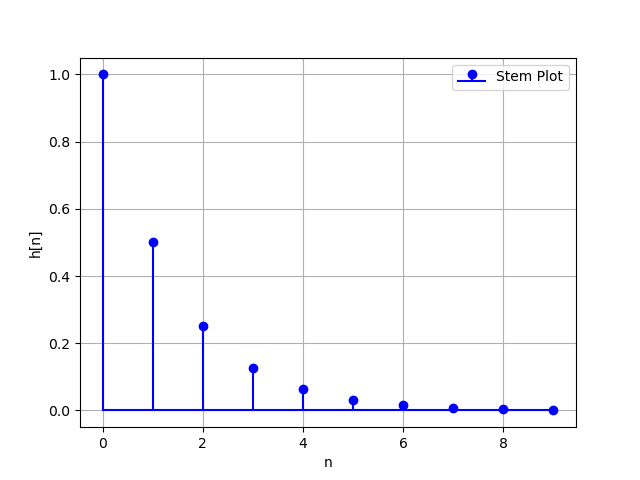
\includegraphics[width=0.5\textwidth]{2023/BM/26/figs/fig1.png}
    \caption{Plot of $h[n]$ vs $n$}
    \label{fig:GATE.2023.BM.26.1}
\end{figure}

\begin{enumerate}
\item From \eqref{eq:GATE.2023.BM.26.6} , \ref{option:GATE.2023.BM.26.1} is wrong
\item As pole lies within unit circle \ref{option:GATE.2023.BM.26.2} is true
\item From \eqref{eq:GATE.2023.BM.26.6} and \figref{fig:GATE.2023.BM.26.1} ,\ref{option:GATE.2023.BM.26.3} is true and hence
\item \ref{option:GATE.2023.BM.26.4} is false 
\end{enumerate}





%\end{document}

\newpage
\item A continuous real-valued signal $x\brak{t}$ has finite positive energy and $x\brak{t} = 0$, $\forall$ $t < 0$. From the list given below, select ALL the signals whose
continuous-time Fourier transform is purely imaginary.\\
\begin{enumerate}
\item$x\brak{t} + x\brak{-t}$
\item$x\brak{t} - x\brak{-t}$
\item$j\brak{x\brak{t} + x\brak{-t}}$
\item$j\brak{x\brak{t} - x\brak{-t}}$
\end{enumerate}
\hfill{(GATE IN 2023)}\\
\solution
\iffalse
\documentclass[journal,12pt,twocolumn]{IEEEtran}
\usepackage{cite}
\usepackage{amsmath,amssymb,amsfonts,amsthm,mathtools}
\usepackage{algorithmic}
\usepackage{graphicx}
\parindent 0px
\bibliographystyle{IEEEtran}
\title{GATE 2023-EE Q49}
\author{EE23BTECH11052 - Abhilash Rapolu}
\begin{document}
\maketitle
\newpage
\textbf{Question 49}: The period of the discrete-time signal x[n] described by the equation below is N =\ (Round off to the nearest integer).
$$x[n] = 1 + 3\sin\left(\frac{15\pi}{8}n + \frac{3\pi}{4}\right) - 5\sin\left(\frac{\pi}{3}n - \frac{\pi}{4}\right)$$
\textbf{Solution:}
\fi
\begin{table}[htbp]
\centering
\begin{tabular}{|l|l|c|}
\hline
\textbf{Parameter} & \textbf{Description} & \textbf{Value} \\
\hline
$f_{1}$ & Sinusoid1 Frequency & 15/16 \\
\hline
$f_{2}$ & Sinusoid2 Frequency & 6 \\
\hline
\end{tabular}

 
\caption{Given parameters list}
\end{table}

The time period must be an integer for a discrete-time signal.
\begin{align}
T_1 &= \frac{1}{f_1} = \frac{16}{15} \\
T_2 &= \frac{1}{f_2} = 6 \\
N &= \text{LCM}(T_1, T_2) = 48
\end{align}

The Time Period of the signal is \(N = 48\).

Let's find the Discrete Fourier Transform (\(X[k]\)):
\begin{align}
X[k] &= \sum_{n=0}^{N-1} x[n]e^{-j\frac{2\pi}{N}kn} \\
X[k] &= \sum_{n=0}^{47} \left(1 + 3\sin\left(\frac{15\pi}{8}n + \frac{3\pi}{4}\right) 
- 5\sin\left(\frac{\pi}{3}n - \frac{\pi}{4}\right)\right) \cdot e^{-j\frac{2\pi}{48}kn} \\
X[k] &= \begin{cases}
    48 & \text{if } k = 0 \\
    50.9117 - 50.9117j & \text{if } k = 3 \\
    0 & \text{otherwise}
\end{cases}
\end{align}

\begin{figure}[!ht] 
\centering
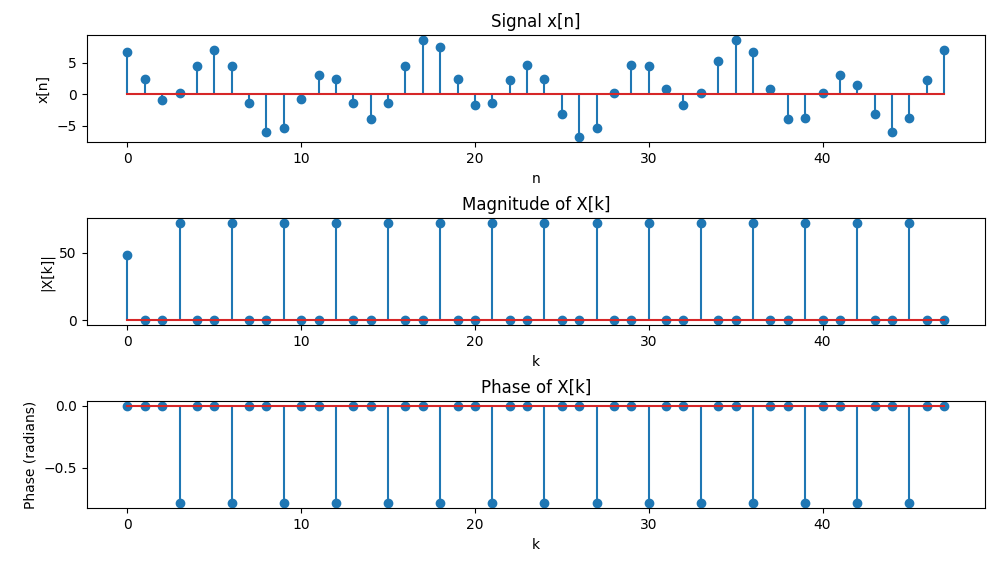
\includegraphics[width=1\columnwidth]{2023/EE/49/figs/Figure1.png}
\label{fig:Graph1}
\end{figure}

%\end{document}










\item Let $x_1(t) = u(t + 1.5) - u(t - 1.5)$ and $x_2(t)$ is shown in the figure below. For $y(t) = x_1(t) * x_2(t)$, the $\int_{-\infty}^{\infty} y(t) \, dt$ is \underline{\hspace{2cm}}.\\

\begin{figure}[htbp]
    \centering
    \includegraphics[width=0.5\textwidth]{2023/EC/58/figs/gatefig.png}
    \caption{Figure}
    \label{fig:graph}
\end{figure}

\hfill{(GATE IN 2023)}\\
\solution
\input{2023/EC/58/gate_ec_58.tex}
\pagebreak
\item Consider a discrete-time signal with period $N=5$. Let the discrete-time Fourier series (DTFS) representation be $ x[n] = \sum\limits_{k=0}^{4} a_k e^{\frac{jk2\pi n}{5}} $where $a_0=1$, $a_1=3j$, $a_2=2j$, $a_3=-2j$, $a_4=-3j$. The value of the sum $\sum\limits_{n=0}^{4}x[n] \sin\left(\frac{4\pi n}{5}\right) $is\\
(A) -10\\
(B) 10\\
(C) -2\\
(D) 2\\
\hfill Gate 2023 EC 47
\solution
\pagebreak

\item A continuous time, band-limited signal $x(t)$ has its Fourier transform described by:
\[ X(f) = \begin{cases} 
1 - \frac{|f|}{200} & \text{if } |f| \leq 200 \\
0 & \text{if } |f| > 200 
\end{cases} \]
The signal is uniformly sampled at a sampling rate of 600 Hz. The Fourier transform of the signal is $X_s(f)$. What is the value of $\frac{X_s(600)}{X_s(500)}$? \\\hfill{(GATE 2023 BM)}
\solution
\iffalse
\let\negmedspace\undefined
\let\negthickspace\undefined
\documentclass[a4,12pt,twocolumn]{IEEEtran}
%\documentclass[conference]{IEEEtran}
%\IEEEoverridecommandlockouts
% The preceding line is only needed to identify funding in the first footnote. If that is unneeded, please comment it out.
\usepackage{cite}
\usepackage{amsmath,amssymb,amsfonts,amsthm}
\usepackage{algorithmic}
\usepackage{graphicx}
\usepackage{textcomp}
\usepackage{xcolor}
\usepackage{txfonts}
\usepackage{listings}
\usepackage{enumitem}
\usepackage{mathtools}
\usepackage{gensymb}
\usepackage[breaklinks=true]{hyperref}
\usepackage{tkz-euclide} % loads  TikZ and tkz-base
\usepackage{listings}
\usepackage{empheq}
\usepackage[utf8]{inputenc}
\usepackage{pgfplots}
\usepackage{mathrsfs}
\usepackage{multicol}
\usepackage{array}
%\usepackage{setspace}
%\usepackage{gensymb}
%\doublespacing
%\singlespacing

%\usepackage{graphicx}

\DeclareMathOperator*{\Res}{Res}
%\renewcommand{\baselinestretch}{2}
\renewcommand\thesection{\arabic{section}}
\renewcommand\thesubsection{\thesection.\arabic{subsection}}
\renewcommand\thesubsubsection{\thesubsection.\arabic{subsubsection}}

\renewcommand\thesectiondis{\arabic{section}}
\renewcommand\thesubsectiondis{\thesectiondis.\arabic{subsection}}
\renewcommand\thesubsubsectiondis{\thesubsectiondis.\arabic{subsubsection}}

% correct bad hyphenation here
\hyphenation{op-tical net-works semi-conduc-tor}
\def\inputGnumericTable{}                                 %%

\lstset{
%language=C,
frame=single, 
breaklines=true,
columns=fullflexible
}
%\lstset{
%language=tex,
%frame=single, 
%breaklines=true
%}

\begin{document}
%


\newtheorem{theorem}{Theorem}[section]
\newtheorem{problem}{Problem}
\newtheorem{proposition}{Proposition}[section]
\newtheorem{lemma}{Lemma}[section]
\newtheorem{corollary}[theorem]{Corollary}
\newtheorem{example}{Example}[section]
\newtheorem{definition}[problem]{Definition}
%\newtheorem{thm}{Theorem}[section] 
%\newtheorem{defn}[thm]{Definition}
%\newtheorem{algorithm}{Algorithm}[section]
%\newtheorem{cor}{Corollary}
\newcommand{\BEQA}{\begin{eqnarray}}
\newcommand{\EEQA}{\end{eqnarray}}
\newcommand{\define}{\stackrel{\triangle}{=}}

\bibliographystyle{IEEEtran}
%\bibliographystyle{ieeetr}


\providecommand{\mbf}{\mathbf}
\providecommand{\pr}[1]{\ensuremath{\Pr\left(#1\right)}}
\providecommand{\qfunc}[1]{\ensuremath{Q\left(#1\right)}}
\providecommand{\sbrak}[1]{\ensuremath{{}\left[#1\right]}}
\providecommand{\lsbrak}[1]{\ensuremath{{}\left[#1\right.}}
\providecommand{\rsbrak}[1]{\ensuremath{{}\left.#1\right]}}
\providecommand{\brak}[1]{\ensuremath{\left(#1\right)}}
\providecommand{\lbrak}[1]{\ensuremath{\left(#1\right.}}
\providecommand{\rbrak}[1]{\ensuremath{\left.#1\right)}}
\providecommand{\cbrak}[1]{\ensuremath{\left\{#1\right\}}}
\providecommand{\lcbrak}[1]{\ensuremath{\left\{#1\right.}}
\providecommand{\rcbrak}[1]{\ensuremath{\left.#1\right\}}}
\theoremstyle{remark}
\newtheorem{rem}{Remark}
\newcommand{\sgn}{\mathop{\mathrm{sgn}}}
%\providecommand{\abs}[1]{\left\vert#1\right\vert}
\providecommand{\res}[1]{\Res\displaylimits_{#1}} 
%\providecommand{\norm}[1]{\left\lVert#1\right\rVert}
%\providecommand{\norm}[1]{\lVert#1\rVert}
\providecommand{\mtx}[1]{\mathbf{#1}}
%\providecommand{\mean}[1]{E\left[ #1 \right]}
\providecommand{\fourier}{\overset{\mathcal{F}}{ \rightleftharpoons}}
%\providecommand{\hilbert}{\overset{\mathcal{H}}{ \rightleftharpoons}}
\providecommand{\system}{\overset{\mathcal{H}}{ \longleftrightarrow}}
	%\newcommand{\solution}[2]{\textbf{Solution:}{#1}}
\newcommand{\solution}{\noindent \textbf{Solution: }}
\newcommand{\cosec}{\,\text{cosec}\,}
\providecommand{\dec}[2]{\ensuremath{\overset{#1}{\underset{#2}{\gtrless}}}}
\newcommand{\myvec}[1]{\ensuremath{\begin{pmatrix}#1\end{pmatrix}}}
\newcommand{\mydet}[1]{\ensuremath{\begin{vmatrix}#1\end{vmatrix}}}
%\numberwithin{equation}{section}
%\numberwithin{equation}{subsection}
%\numberwithin{problem}{section}
%\numberwithin{definition}{section}
%\makeatletter
%\@addtoreset{figure}{problem}
%\makeatother

%\let\StandardTheFigure\thefigure
\let\vec\mathbf

\title{
\Huge\textbf{Gate EE 2023}\\
\Huge\textbf{EE1205} Signals and Systems\\
}
\large\author{Nimal Sreekumar\\EE23BTECH11044}

% make the title area
\maketitle


%\tableofcontents

\bigskip

\renewcommand{\thefigure}{\arabic{figure}}
\renewcommand{\thetable}{\theenumi}
%\renewcommand{\theequation}{\theenumi}


\textbf{Question Gate 2023 EE:}
For the signals x\brak{t} and y\brak{t} shown in the figure, $z\brak{t}=x\brak{t}*y\brak{t}$ is maximum at $t=T_1$. Then $T_1$ in seconds is .......... \brak{\text{Round off to the nearest integer}}\\

\begin{tikzpicture}
\begin{axis}[xmin=-3, xmax=7, ymin=-3, ymax=3, axis lines=middle, xlabel={$t$}, title={$y\brak{t}$}]
 \addplot[blue] coordinates {(-3,0) (1,0)};
  \addplot[blue] coordinates {(1,0) (1,-2)};
   \addplot[dashed] coordinates {(0,-2) (1,-2)};
  \addplot[blue, domain=1:5] {x - 3};
  \addplot[blue] coordinates {(5,2) (5,0)};
  \addplot[blue] coordinates {(5,0) (7,0)};
  \addplot[dashed] coordinates {(0,2) (5,2)};
    \end{axis}
\end{tikzpicture}

\begin{tikzpicture}
    \begin{axis}[xmin=-3, xmax=3, ymin=-3, ymax=3, axis lines=middle, xlabel={$t$} ,title={$x\brak{t}$}]
        \addplot[blue] coordinates {(-3,0) (-1,0)};
        \addplot[blue] coordinates {(-1,0) (-1,1)};
        \addplot[blue] coordinates {(-1,1) (1,1)};
        \addplot[blue] coordinates {(1,1) (1,0)};
        \addplot[blue] coordinates {(1,0) (3,0)};
    \end{axis}
\end{tikzpicture}

\hfill (GATE EE 2023)
\solution
\fi

\begin{table}[htbp]
\centering
\renewcommand\thetable{1}
\begin{tabular}{|c|m{3.5cm}|m{3cm}|}
    \hline
    \textbf{Variable} & \textbf{values} & \textbf{Description} \\
    \hline
    $x\brak{t}$ & $u\brak{t+1}-u\brak{t-1}$ & signal 1\\
    \hline
    $ y\brak{t} $ & $y\brak{t} = 
    \begin{cases}
        t-3 & ; 1\leq n \leq 5 \\
        0 & ; otherwise \\
    \end{cases}$ & signal 2\\
    \hline
    $X\brak{s}$ & $\int_{0}^{\infty}x\brak{t}e^{-st}dt$ & Laplace transform of $x\brak{t}$\\
    \hline
   $Y\brak{s}$ & $\int_{0}^{\infty}y\brak{t}e^{-st}dt$ & Laplace transform of $y\brak{t}$ \\
    \hline
    $\mathscr{L^{-1}} \{Z(s)\}$ &$f\brak{t-c}u\brak{t-c}=\mathscr{L^{-1}}\brak{e^{-cs}F\brak{s}} $& Inverse Laplace transform \\
    \hline
\end{tabular}
\caption{Input Parameters}
\label{tab:11.9.5.32}
\end{table}

Using laplace transform,
\begin{align}
z\brak{t} &=x\brak{t}*y\brak{t}\label{eq:gate_ee_Q31.1} \\
Z\brak{s} &=X\brak{s}Y\brak{s}\label{eq:gate_ee_Q31.2} \\
X\brak{s} &= \frac{1}{s} \brak{e^{s}-e^{-s}} \label{eq:gate_ee_Q31.3}\\
Y\brak{s} &= \frac{2s+1}{s^2} \brak{e^{-s}-e^{-5s}}\label{eq:gate_ee_Q31.4}\\
Z\brak{s} &= \frac{2s+1}{s^3} \brak{1-e^{-4s}-e^{-2s}+e^{-6s}}\label{eq:gate_ee_Q31.5}
\end{align}
Now taking inverse laplace transform for each terms, $\mathscr{L^{-1}} \{Z(s)\}$
\begin{align}
&= \left( 2t + \frac{t^2}{2} \right) u(t) \nonumber \\
&\quad - \left( 2(t-4) + \frac{(t-4)^2}{2} \right)u(t-4) \nonumber \\
&\quad - \left( 2(t-2) + \frac{(t-2)^2}{2} \right)u(t-2) \nonumber \\
&\quad + \left( 2(t-6) + \frac{(t-6)^2}{2} \right)u(t-6) \nonumber
\end{align}\label{eq:gate_ee_Q31.6}
From the plot it is clear that $T_1=4$.\\
\begin{figure}[h]
\centering
   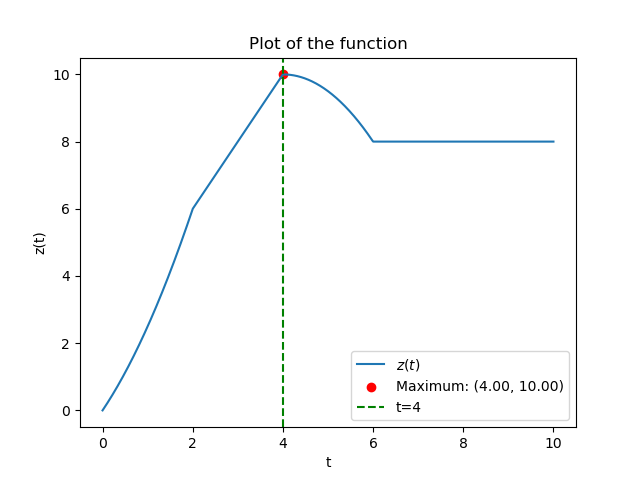
\includegraphics[width=1\linewidth]{2023/EE/31/figs/figs/gate2023EE.png}
   \caption{z\brak{t} vs. t}
   \label{fig:gate2023EE1}
 \end{figure}\\
Now in time domain,
 \begin{align}
z\brak{t} &=x\brak{t}*y\brak{t} = y\brak{t}*x\brak{t}\label{eq:gate_ee_Q31.7}\\
z\brak{t} &=\int_{-\infty}^{\infty} y\brak{\tau}x\brak{t-\tau}d\tau\label{eq:gate_ee_Q31.8}
\end{align}
$x\brak{\tau}$ is an even signal,
\begin{align}
x\brak{\tau}= x\brak{-\tau}\label{eq:gate_ee_Q31.9}\\
 x\brak{-\tau}= 
    \begin{cases}
        1 & ; -1\leq -\tau \leq 1 \\
        0 & ; \text{otherwise} \\
    \end{cases}\label{eq:gate_ee_Q31.10}
    \end{align}
    
    \begin{align}
    x\brak{-\tau} \xleftrightarrow{\text{Time shifting}} x\brak{t-\tau}\label{eq:gate_ee_Q31.11} \\
    x\brak{t-\tau}= 
    \begin{cases}
        1 & ; t-1\leq t-\tau \leq t+1 \\
        0 & ; \text{otherwise} \\
    \end{cases}\label{eq:gate_ee_Q31.12}
\end{align}\\
For $z\brak{t}$ to be maximum both $y\brak{\tau}$ and $x\brak{t-\tau}$ must be maximum,
\begin{align}
\implies t-1 &= 3 \quad \text{or} \quad t+1 = 5 \nonumber \\
t &= T_1 = 4 \nonumber
\end{align}

\pagebreak

 \item The magnitude and phase plots of an LTI systems are shown in figure. Find the transfer function.
\begin{figure}[!h]
    \centering
    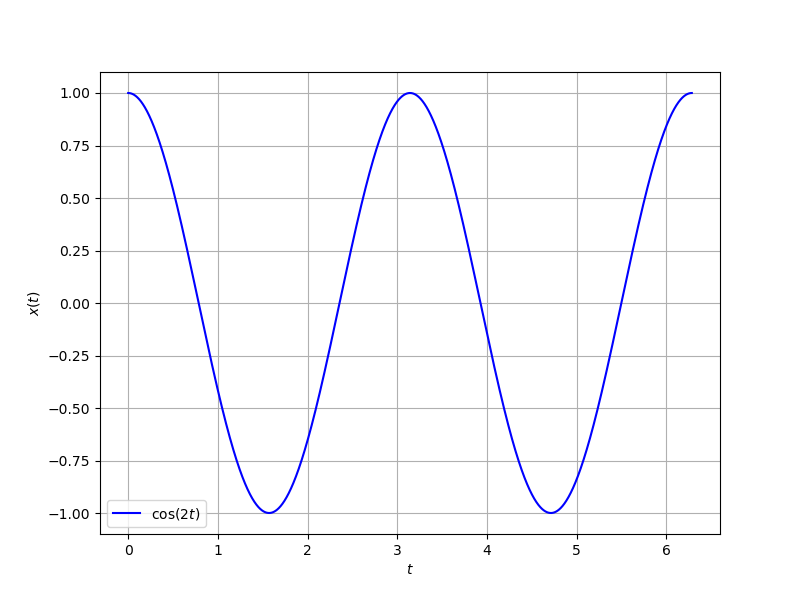
\includegraphics[width=\columnwidth]{2023/EE/36/figs/gate.png}
    \caption{}
    \label{fig:EEgatefig36.23}
\end{figure}
\begin{enumerate}
    \item $2.511 e^{-0.0032s}$\\
    \item $\frac{e^{-2.514s}}{s+1}$\\
    \item $1.04e^{-2.514s}$\\
    \item $2.511 e^{-1.047s}$\\
\end{enumerate} \hfill{(GATE EE 23)}\\

\solution
\input{2023/EE/36/36.tex}
\newpage
\item The value of the convolution of $f(x) = 3\cos(2x)$ and $g(x) = \frac{1}{3}\sin(2x)$ where $x \in [0, 2\pi)$, at $x = \frac{\pi}{3}$, is (Rounded off to 2 decimal places)\\
\hfill (GATE 2023 GE)\\
\solution
\pagebreak
\item A system is described by the following differential equation
    \[
    0.01 \frac{d^2y(t)}{dt^2} + 0.2\frac{dy(t)}{dt} + y(t) = 6x(t)
    \]
    where time \( t \) is in seconds. If \( x(t) \) is the unit step input applied at \( t = 0 \) s to this system, the magnitude of the output at \( t = 1 \) s is \(\underline{\hspace{2cm}}\). (Round off the answer to two decimal places.)
    \hfill (GATE-2023.BM)\\
    \solution
     \iffalse
\let\negmedspace\undefined
\let\negthickspace\undefined
\documentclass[journal,12pt,twocolumn]{IEEEtran}
\usepackage{amssymb}
\usepackage{cite}
\usepackage{amsmath,amssymb,amsfonts,amsthm}
\usepackage{algorithmic}
\usepackage{graphicx}
\usepackage{textcomp}
\usepackage{xcolor}
\usepackage{txfonts}
\usepackage{listings}
\usepackage{enumitem}
\usepackage{mathtools}
\usepackage{gensymb}
\usepackage{comment}
\usepackage[breaklinks=true]{hyperref}
\usepackage{tkz-euclide} 
\usepackage{listings}
\usepackage{gvv}                                        
\def\inputGnumericTable{}                                 
\usepackage[latin1]{inputenc}                                
\usepackage{color}                                            
\usepackage{array}                                            
\usepackage{longtable}                                       
\usepackage{calc}                                             
\usepackage{multirow}                                         
\usepackage{hhline}                                           
\usepackage{ifthen}                                           
\usepackage{lscape}
\usepackage{pgfplots}
\newtheorem{theorem}{Theorem}[section]
\newtheorem{problem}{Problem}
\newtheorem{proposition}{Proposition}[section]
\newtheorem{lemma}{Lemma}[section]
\newtheorem{corollary}[theorem]{Corollary}
\newtheorem{example}{Example}[section]
\newtheorem{definition}[problem]{Definition}
\newcommand{\BEQA}{\begin{eqnarray}}
\newcommand{\EEQA}{\end{eqnarray}}
\newcommand{\define}{\stackrel{\triangle}{=}}
\theoremstyle{remark}
\newtheorem{rem}{Remark}
\begin{document}

\bibliographystyle{IEEEtran}
\vspace{3cm}

\title{GATE 2023-BM.54}
\author{EE22BTECH11004 - Allu Lohith}

\maketitle

    A system is described by the following differential equation
    
    $$\brak{0.01} \frac{d^2y\brak t}{dt^2} + \brak{0.2}\frac{dy\brak t }{dt} + y\brak t = 6x\brak t$$
    where time $t$ is in seconds. If $x\brak t$ is the unit step input applied at $t = 0$ s to this system, the magnitude of the output at $t = 1$s is $\underline{\hspace{2cm}}$. (Round off the answer to two decimal places.)\\

    \hfill {GATE 2023-BM.54}
    
\solution
\fi
\begin{table}[h!]
\centering
\renewcommand{\arraystretch}{2}
\begin{tabular}{|c|p{4cm}|c|}
\hline 
\textbf{Parameter} & \textbf{Description} & \textbf{Formulae/Value} \\
\hline
$x\brak t$ & The unit step input applied at $t = 0$ s to this system & $\begin{cases}
0, & \text{if } t < 0, \\
1, & \text{if } t \geq 0.
\end{cases}$ \\
\hline
$y \brak t$ & A function of $x\brak t$ & - \\
\hline
$y\brak 1$ & Value of $y$ at $t=1$ & -\\
\hline
\end{tabular}

\vspace{0.5cm}
\caption{\normalsize Parameters}
\end{table}
    Given,
    \begin{align}
         \brak{0.01} \frac{d^2y\brak t}{dt^2} + \brak{0.2}\frac{dy\brak t }{dt} + y\brak t = 6x\brak t
    \end{align}
    property:
    \begin{align}
        \mathcal{L}\left\{\frac{d^n y\brak t}{dt^n}\right\} = s^n Y\brak s - s^{n-1} y\brak 0 - \dots - y^{\brak{n-1}}\brak 0
    \end{align}
    Taking the Laplace transform of both sides (assuming zero initial conditions):
   \begin{align}
        0.01s^2Y\brak s + 0.2sY\brak s + Y\brak s = \frac{6}{s}
    \end{align}
    \begin{align}
        \implies Y\brak s &= \frac{6}{s\brak{0.01s^2 + 0.2s + 1}}\\
        \implies Y\brak s &= \frac{6}{ 0.01\brak s \brak {s + 10}^2}
    \end{align}
    Using partial fraction decomposition:
    \begin{align}
    Y\brak s = \frac{A}{s} + \frac{B}{s + 10} + \frac{C}{\brak {s + 10}^2}
    \end{align}
    On solving, we get $A=6,B=-6,C=-60$.\\
    So,\begin{align}
        Y\brak s = \frac{6}{s} - \frac{6}{s + 10} - \frac{60}{\brak {s + 10}^2}
    \end{align}
    From standard inverse laplace transforms:
    \begin{align}
	    \frac{1}{s+a}   &{\longleftrightarrow}    e^{-at}\\
	    \frac{1}{\brak{s+a}^2}  &{\longleftrightarrow }  te^{-at}
    \end{align}	    
	    
    Taking inverse Laplace transform of $Y\brak s$,
    \begin{align}
	    y\brak t &= u\brak{t} \brak{6-6e^{-10t}-60te^{-10t}}
    \end{align}
    At $t=1s$ 
    \begin{align}
        y\brak 1 &=u\brak 1 \brak{6-66e^{-10}}\\
        y\brak 1 &=6-66e^{-10}
    \end{align}
    approximately,
    \begin{align}
	    \implies y\brak{1} =5.99
    \end{align}
    
   \begin{figure}[h]
    \centering  

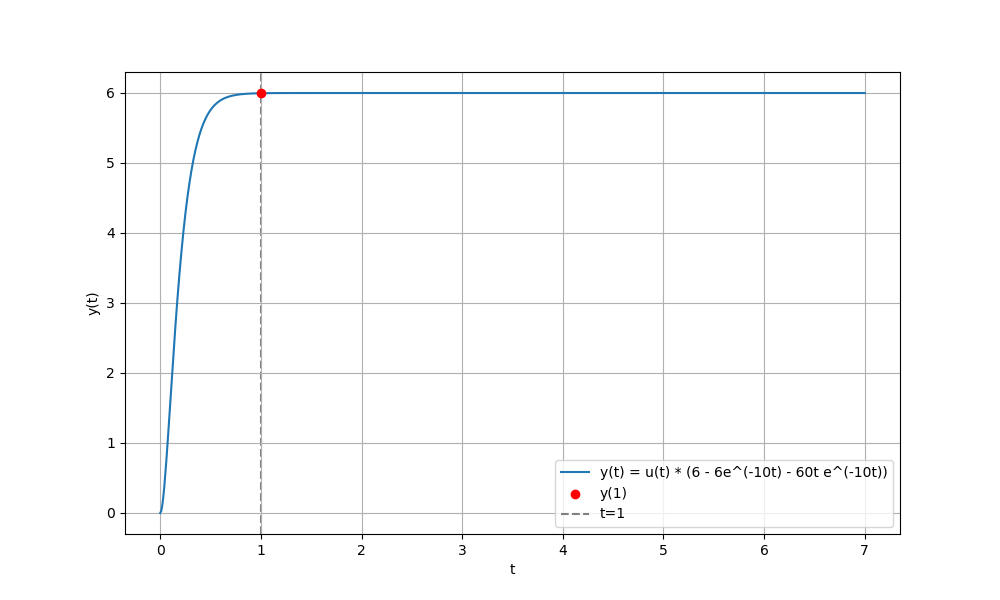
\includegraphics[width=\columnwidth]{2023/BM/54/figs/plot.png}

    \centering
    \caption{Plot of $y\brak t = u\brak t \brak{6-6e^{-10t}-60te^{-10t}}$}
\end{figure}


    \pagebreak

\item In the differential equation $\frac{dy}{dx} + \alpha x y = 0, \alpha$ is a positive constant. If $y = 1.0$ at
$x = 0.0$, and $y = 0.8$ at $x = 1.0$, the value of $\alpha$ is (rounded off to three decimal places).  \hfill(GATE CE 30 2023)\\
\solution
\iffalse
\let\negmedspace\undefined
\let\negthickspace\undefined
\documentclass[journal,12pt,twocolumn]{IEEEtran}
\usepackage{cite}
\usepackage{amsmath,amssymb,amsfonts}
\usepackage{graphicx}
\usepackage{textcomp}
\usepackage{xcolor}
\usepackage{txfonts}
\usepackage{listings}
\usepackage{enumitem}
\usepackage{mathtools}
\usepackage{gensymb}
\usepackage{comment}
\usepackage[breaklinks=true]{hyperref}
\usepackage{tkz-euclide} 
\usepackage{listings}
\usepackage{gvv}                                        
\def\inputGnumericTable{}                                 
\usepackage[latin1]{inputenc}                                
\usepackage{color}                                            
\usepackage{array}                                            
\usepackage{longtable}                                       
\usepackage{calc}                                             
\usepackage{multirow}                                         
\usepackage{hhline}                                           
\usepackage{ifthen}                                           
\usepackage{lscape}
\usepackage[export]{adjustbox}

\newtheorem{theorem}{Theorem}[section]
\newtheorem{problem}{Problem}
\newtheorem{proposition}{Proposition}[section]
\newtheorem{lemma}{Lemma}[section]
\newtheorem{corollary}[theorem]{Corollary}
\newtheorem{example}{Example}[section]
\newtheorem{definition}[problem]{Definition}
\newcommand{\BEQA}{\begin{eqnarray}}
\newcommand{\EEQA}{\end{eqnarray}}
\newcommand{\define}{\stackrel{\triangle}{=}}
\newtheorem{rem}{Remark}

\begin{document}
\parindent 0px
\bibliographystyle{IEEEtran}

\vspace{3cm}

\title{}
\author{EE23BTECH11042 -  Khusinadha Naik$^{*}$
}
\maketitle
\newpage
\bigskip

% \renewcommand{\thefigure}{\theenumi}
% \renewcommand{\thetable}{\theenumi}


\noindent \textbf{26.} \hspace{2pt}A causal, discrete time system is described by the difference equation $y[n] = 0.5 y[n-1] + x[n]$, for all $n$, where $y[n]$ denotes the output sequence and $x[n]$ denotes the input sequence. Which of the following statements is/are TRUE?
\begin{flushright}
\hfill(GATE 2023 BM)
\end{flushright}
\begin{enumerate}[label = (\alph*)]
	\item The system has an impulse response described by $0.5^{n} u[-n]$ where $u[n]$ is the  
unit step sequence. 	\label{option:GATE.2023.BM.26.1}	
	\item The system is stable in the bounded input, bounded output sense.		\label{option:GATE.2023.BM.26.2}
	\item The system has an infinite number of non-zero samples in its impulse response	\label{option:GATE.2023.BM.26.3}
	\item The system has a finite number of non-zero samples in its impulse response.	\label{option:GATE.2023.BM.26.4}
\end{enumerate}

\noindent \textbf{Ans.}\\
\fi
\begin{table}[h]
\centering
\begin{tabular}{|c|c|c|}
        \hline
        \textbf{Parameter} & \textbf{Value} & \textbf{Description} \\
        \hline
        $x[n]$ & ? & Input Sequence \\
        \hline
        $y[n]$ & ? & Output Sequence \\
        \hline
\end{tabular}
\caption{Input parameters table}
\label{tab:GATE.2023.BM.26.1}





\end{table}
\begin{align}
y[n] = 0.5y[n-1] + x[n] 
\end{align}

Taking $Z$-Transform 
\begin{align}
Y\brak{z} &= 0.5z^{-1}Y\brak{z} + X\brak{z} \\
\implies \frac{Y\brak{z}}{X\brak{z}} &= \frac{1}{1 - 0.5z^{-1}} = H\brak{z} 
\end{align}
If $x[n]$ is impulse input 
\begin{align}
\implies &Y\brak{z} = H\brak{z} = \frac{1}{1 - 0.5z^{-1}}  \label{eq:GATE.2023.BM.26.4}
\end{align}
From \eqref{eq:GATE.2023.BM.26.4} pole lies at $z = 0.5$
\begin{align}
a^{n}u\brak{n} \xleftrightarrow{\mathcal{Z}} &\frac{1}{1 - az^{-1}} \quad , \abs{z} > a \label{eq:GATE.2023.BM.26.5}
\end{align}

From \eqref{eq:GATE.2023.BM.26.4} , \eqref{eq:GATE.2023.BM.26.5}
\begin{align}
h[n] = 0.5^{n}u[n] \quad , \abs{z} > 0.5 \label{eq:GATE.2023.BM.26.6}
\end{align}


\pagebreak
Plotting $h[n]$ vs $n$
\begin{figure}[h]
    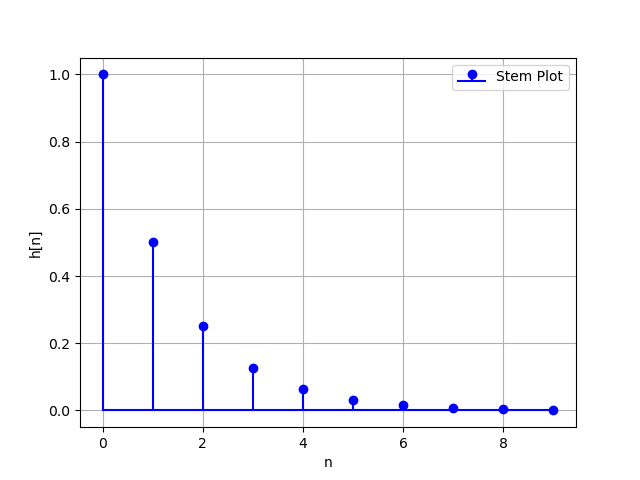
\includegraphics[width=0.5\textwidth]{2023/BM/26/figs/fig1.png}
    \caption{Plot of $h[n]$ vs $n$}
    \label{fig:GATE.2023.BM.26.1}
\end{figure}

\begin{enumerate}
\item From \eqref{eq:GATE.2023.BM.26.6} , \ref{option:GATE.2023.BM.26.1} is wrong
\item As pole lies within unit circle \ref{option:GATE.2023.BM.26.2} is true
\item From \eqref{eq:GATE.2023.BM.26.6} and \figref{fig:GATE.2023.BM.26.1} ,\ref{option:GATE.2023.BM.26.3} is true and hence
\item \ref{option:GATE.2023.BM.26.4} is false 
\end{enumerate}





%\end{document}

\pagebreak

\end{enumerate}
